\chapter{Background}\label{ch:2}

\begin{remark}{Outline}
\todo{change outline}
In this chapter, we introduce classifications models from a machine learning perspective. 
Moreover, we present the example-dependent cost-sensitive framework that is the basis of the 
thesis. In Section~\ref{sec:2:classification}, we give a self contain introduction to 
classification, including the most-common algorithms, and the main methods for evaluating the 
performance of the different algorithm. Then, in Section~\ref{sec:2:cs}, we present the general 
framwork of cost-sensitive classification. Within this Section, we first introduce a method for 
defining the type of cost-sensitivity of a problem. Afterwards, we present the different 
cost-sensitive performance evaluation measures. Lastly, we show the state-of-the-art 
example-dependent cost-sensitive methods cost-proportionate rejection-sampling and 
cost-proportionate over-sampling.
\end{remark}

\section{Basics on classification}
\label{sec:2:classification}

In machine learning, classification refers to the attempt of identifying to which of a set of 
classes a new example belongs, based on learning from examples whose class membership is known. 
The most important point about classification is that for each example only one know class is 
possible, making this a discrete problem. 

A classification, task begins with a training set in which the class of a set of examples is know. 
For example, a classification model that predicts credit card fraud, is developed by analyzing 
many observed credit transactions over a period of time. The class in this case is a variable which 
indicates for each example whether or not the transaction was o not a fraud. Also, the predictors 
or features, are the transaction attributes like place, amount and time of the transaction.

Then, during the training process, a classification algorithm finds the patterns and relationships 
between the values of the features and the values of the target class. Different algorithms use 
different methods and techniques to estimate the relationships. Afterwards, these relationships are 
summarized in a model that is able to make predictions on new sets of data.

Formally, a classification algorithm deals with the problem	of predicting the class $y_i$ of a 
set $\mathcal{S}$ of examples or instances, given their $k$ features \mbox{$\mathbf{x}_i \in 
\mathbb{R}^k$}. The objective is to construct a function $f(\cal{S})$ that makes a prediction 
$c_i$ of the class of each of the $N$ examples using its feature vector $\mathbf{x}_i$.
Moreover, some algorithms allows to not only know the prediction, but also the confidence of it, in 
the form of the probability of belonging to the positive class $\hat p_i$. The way for going from 
$\hat p_i$ to $c_i$, is simply by defining a probability threshold $t$, and applying the following 
formula
\begin{equation}\label{eq_pred}
  c_i = 
  \begin{cases}
    \phantom{-}0 \phantom{-} \mbox{if} \phantom{-} \hat p_i \le t\\
    \phantom{-}1 \phantom{-}\mbox{otherwise,}
  \end{cases}
\end{equation}
Usually, $t=\frac{1}{2}$ \citep{Hastie2009}, as an example with probability of being positive 
higher than 50\% is classified as positive, and negative otherwise. If $t \ne \frac{1}{2}$, the 
function that generates the predicted class labels $\mathbf{c}$ is refers as $f^t$.

\begin{figure}
	\centering
	  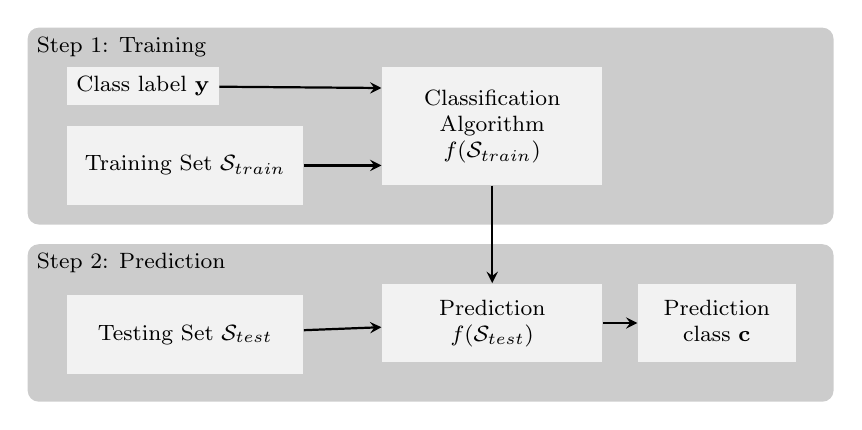
\begin{tikzpicture}[node distance=2cm]
  \tikzstyle{every node}=[font=\footnotesize]
  
  % Main boxes
  \node (step1) [rectangle, rounded corners, anchor=north west, fill=black!20, text width=10cm,
								minimum height=2.5cm] {};
	\node [anchor=north west] at (step1.north west){Step 1: Training};
	\node (step2) [rectangle, rounded corners, anchor=west, fill=black!20, text width=10cm, 
								minimum height=2cm, below of = step1, yshift=-0.5cm] {};
	\node [anchor=north west] at (step2.north west){Step 2: Prediction};
	
	% Training
	\node (label) [rectangle, anchor=north west, fill=black!5,
								yshift=-0.5cm, xshift=0.5cm] {Class label $\bf y $};
	\node (train) [rectangle, anchor=north west, fill=black!5, minimum height=1cm, minimum width=3cm,
								yshift=-1.25cm, xshift=0.5cm] {Training Set $\mathcal{S}_{train} $};
	\node (algo) [rectangle, anchor=north west, fill=black!5, minimum height=1.5cm,
							 minimum width=2.8cm, yshift=-.50cm, xshift=4.5cm] 
							 {\tabular{c} Classification \\ Algorithm  \\	$f(\mathcal{S}_{train}) $
								\endtabular}; 

	%Classification
	\node (test) [rectangle, anchor=north west, fill=black!5, minimum height=1cm, minimum width=3cm,
								yshift=-3.4cm, xshift=0.5cm] {Testing Set $\mathcal{S}_{test} $};
	\node (algo2)[rectangle, anchor=north west, fill=black!5, minimum height=1cm, minimum width=2.8cm,
							 yshift=-3.25cm, xshift=4.5cm] 
							 {\tabular{c} Prediction \\	$f(\mathcal{S}_{test}) $\endtabular};
	\node (pred) [rectangle, anchor=north west, fill=black!5, minimum height=1cm,
							yshift=-3.25cm, xshift=7.75cm] {\tabular{c} Prediction \\ class $\bf c$	\endtabular};
	
	% Arrows
	\node (label_temp) [rectangle, anchor=north west, yshift=-0.65cm, xshift=4.5cm] {};
	\draw[thick,->,>=stealth] (label) to (label_temp);
	\node (train_temp) [rectangle, anchor=north west,minimum height=1cm, minimum width=3cm,
								yshift=-1.25cm, xshift=4.5cm] {};
	\draw[thick,->,>=stealth] (train) to (train_temp);
	\draw[thick,->,>=stealth] (algo) to (algo2);
	\draw[thick,->,>=stealth] (test) to (algo2);
	\draw[thick,->,>=stealth] (algo2) to (pred);
  \end{tikzpicture}
 
  \caption{Classification process}
  \label{fig:2:1}
\end{figure}

In \figurename{ \ref{fig:2:1}}, the process of a training and using a classification algorithm is 
summarized. First, during the training phase, using a training set $\mathcal{S}_{train}$, a 
algorithm is train to predict $\mathbf{y}$. Then the algorithm is used to make estimate the class 
$\mathbf{c}$ of a set of testing examples $\mathcal{S}_{test}$.

\begin{figure}[!t]
\centering
\subfloat[]{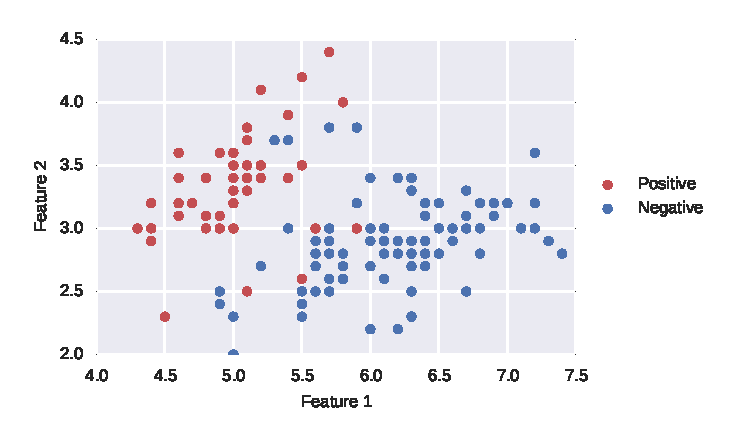
\includegraphics{ch2_fig1a}\label{fig:2:2a}}
\\
\subfloat[]{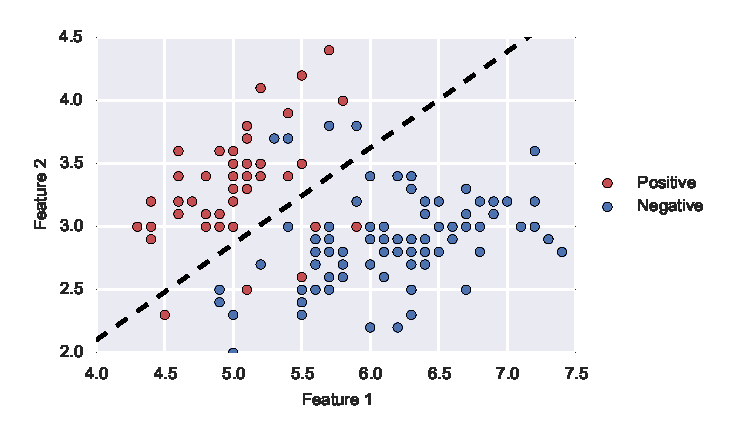
\includegraphics{ch2_fig1b}\label{fig:2:2b}}
\caption{Example of a classification algorithm. Using a set of examples from two classes, a 
	classification algorithm is learn in order to separate between the positives and the negatives. }
\label{fig:2:2}
\end{figure} 

There exists several algorithms that can be used for classification tasks. In general a 
classification algorithm is learn with the objective of finding patterns that separate between the 
different classes \citep{Hastie2009}. In order to clarify this intuition, in \figurename{ 
\ref{fig:2:2}} an example of a classification algorithm is shown. Lets suppose a set of examples as 
shown in \figurename{ \ref{fig:2:2a}}.  Where the red points represents the positive examples and 
the blue the negative examples. The objective of a classifier is to find the best way to separate 
between the positive and negatives examples. In \figurename{ \ref{fig:2:2b}}, the output of a 
classifier learned using the set of examples is shown. It is observed that this classifier is able 
to separate almost all the examples using a linear classifier. 

However, not all examples are correctly classified. In particular there are four negative examples 
that were predicted as positive, and five positive examples that were predicted as negative. In the 
next section, we present the standard methods for evaluating the performance of a classification 
algorithm.

\begin{remark}{Classification examples}
Classification algorithms are widely used across a variety of domains. For example in the 
medical field, models have been used for making predictions about tumors, probability 
of a disease, selecting the right drug for a particular patient, and estimating the probability of 
relapsing, among others \citep{Herland2014}. In the financial sector, classification models have 
been successfully applied for fraud detection, credit scoring, portfolio management and algorithmic 
trading. Also, in marketing, several models are being currently used for churn modeling, customer 
targeting, behavior prediction and direct marketing \citep{Baesens2014}. Additionally, in many 
other emerging applications such as terrorism prevention, malware detection, computer security, 
energy consumption prediction, spam classification, and others \citep{Kriegel2007}.
\end{remark}


\section{Performance measures}

When evaluating the performance of a classification algorithm, the first thing to do is to check 
the number of examples that were misclassified. Since the the true class of the training examples 
is known. Therefore, evaluating the error of a model is as simply as counting the number of times 
an example is misclassified and divide it by the number of examples
\begin{equation}\label{eqn:ch2:error}
Err(f({\cal S})) = \frac{1}{N}  \sum_{i=1}^N \mathbf{1}_{y_i}(c_i),
\end{equation}
where $\mathbf{1}_c(z)$ is an indicator function that takes the value of one if $z \in c$ and 
zero if $z \notin c$. Moreover the accuracy is defined as the percentage of times the algorithm 
made the correct prediction
\begin{equation}\label{eqn:2:accuracy}
Acc(f({\cal S})) = 1- Err(f({\cal S})).
\end{equation}

However, just knowing these statistics is not enough to make decisions, as in many applications is 
important to know where the errors are coming from. In particular, the misclassified examples may 
belong only to one class, which may give interesting insights about the problem. A way to observe 
the different errors is by looking to the confusion matrix, as shown in 
\mbox{\tablename{~\ref{tab:2:1}}}. Afterwards, using the cost matrix several statistics are 
extracted. In particular:
  \begin{flalign}
    &Recall = \frac{TP}{TP+FN} &\\
    &Precision = \frac{TP}{TP+FP}& \\
    &F_1Score = 2\frac{Precision \cdot Recall}{Precision + Recall}&
  \end{flalign}
  
	\begin{table}[!t]
		\centering
		\footnotesize
    \begin{tabular}{c|c|c}
      \multicolumn{3}{c}{}\\
			\multicolumn{1}{c|}{}  & Actual Positive& Actual Negative \\
			\multicolumn{1}{c|}{} & $y=1$& $y=0$ \\
			\hline
			Predicted Positive 		& \multirow{ 2}{*}{True Positive ($TP$)} & \multirow{ 
			2}{*}{False Positive ($FP$)} \\
			$c=1$ & &\\
			\hline
			Predicted Negative  	& \multirow{ 2}{*}{False Negative ($FN$)} & \multirow{ 
			2}{*}{True Negative ($TN$)} \\
			$c=0$ & &\\
		\end{tabular}
		\caption{Classification confusion matrix}
		\label{tab:2:1}
  \end{table}  
 
  As an illustrative example, the different statistics are calculated for the toy example presented 
  in Section~\ref{sec:2:classification}. First, the confusion matrix is calculated as 
  follows:
  \begin{center}
    \footnotesize
  \begin{tabular}{c|c|c}
    \multicolumn{1}{c|}{}  & Actual Positive& Actual Negative \\
    \multicolumn{1}{c|}{} & $y=1$& $y=0$ \\
    \hline
    Predicted Positive    & \multirow{ 2}{*}{36} & \multirow{ 
    2}{*}{4} \\
    $c=1$ & &\\
    \hline
    Predicted Negative    & \multirow{ 2}{*}{5} & \multirow{ 
    2}{*}{68} \\
    $c=0$ & &\\
  \end{tabular}
  \end{center}
  Then using the confusion matrix, the statistics are calculated,
 	\begin{itemize}
  	\item Error = $\frac{4+9}{36+4+9+68}=11.11\%$
		\item Recall = $\frac{TP}{TP+FN}=87.8\%$
		\item Precision = $\frac{TP}{TP+FP}=90\%$
		\item $F_1Score = 2\frac{Precision \cdot Recall}{Precision + Recall}=88.8\%$
	\end{itemize}
	
\begin{figure}[t!]
	\centering
	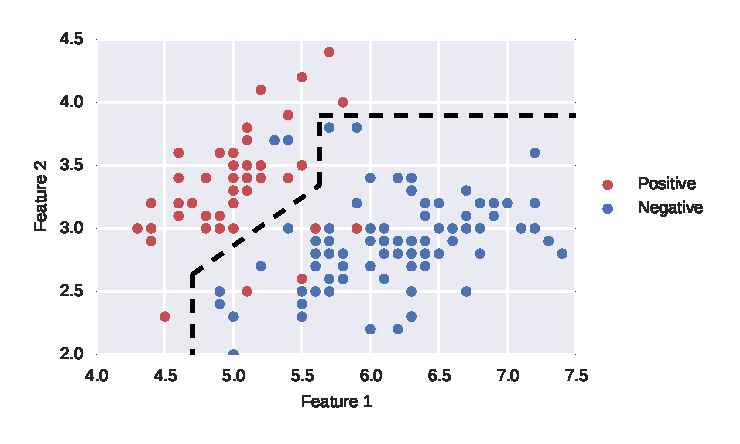
\includegraphics{ch2_fig2}
	\caption{Example of a classification algorithm. Using a set of examples from two classes, a 
	classification algorithm is learn in order to separate between the positives and the negatives. }
	\label{fig:2:3}
\end{figure}

There are however, several instances that are misclassified, thats because the simple linear 
classifier that were used in this example may not be good enough to separate between the positive 
and negative classes. In order to make a comparison, using the same example toy set, a new 
algorithm is learn. This time the algorithm made the correct prediction more often as shown in 
\figurename{ \ref{fig:2:3}}. Afterwards, the confusion matrix and the different statistics are 
calculated as follows:
\begin{center}
		\footnotesize
    \begin{tabular}{c|c|c}
			\multicolumn{1}{c|}{}  & Actual Positive& Actual Negative \\
			\multicolumn{1}{c|}{} & $y=1$& $y=0$ \\
			\hline
			Predicted Positive 		& \multirow{ 2}{*}{37} & \multirow{ 
			2}{*}{2} \\
			$c=1$ & &\\
			\hline
			Predicted Negative  	& \multirow{ 2}{*}{4} & \multirow{ 
			2}{*}{70} \\
			$c=0$ & &\\
		\end{tabular}
\end{center}
  \begin{itemize}
    \item Error = $\frac{4+9}{36+4+9+68}=5.3\%$
    \item Recall = $\frac{TP}{TP+FN}=90.2\%$
    \item Precision = $\frac{TP}{TP+FP}=94.9\%$
    \item $F_1Score = 2\frac{Precision \cdot Recall}{Precision + Recall}=92.5\%$
  \end{itemize}
It is observed that in this case the FP are reduced more than the FN, this leads to a higher 
increase in precision  than in recall. There is not a single rule regarding which one is more 
important to increase, it depends on the applications. For example in applications with a high 
false negative cost such as failing to identify a tumor in a medical exam, the recall should be the 
priority, even if that implies having a significant number of false positives. On the other hand, 
In applications such as spam detection, predicting a normal email as spam, may have a big impact to 
the customer, therefore, in this example is better to allow some false negatives and focus on the 
false positives.

It is not always straightforward  to define the define the right tradeoff between false positives 
and false negatives. The best approximation to solve that, is to focus on the actual costs incurred 
by the different decisions, this is usually solved using cost-sensitive classification methods. A 
deep analysis of these methods is described in the following Section.

\subsection{Brier score}
\label{sec:2:brier}

Traditional evaluation measures of binary classification problems, such as Accuracy and 
$F_1Score$, provide a way to analyze the performance of a model. However, when using the classifier 
output as a basis for decision making, there is a need of a measure that takes into account not 
only the misclassification of a classifier $\mathbf{c}$, but also the quality of the estimated 
probability $\mathbf{\hat p}$ \citep{cohen2004}. The most appropriate  is the Brier score 
\citep{brier1950}. The Brier score is one of a class of so-called proper scores which are used in 
evaluating the subjective probability assessment of forecasters \citep{DeGroot1983}. The Brier 
score is the average squared difference between the forecasters estimated probability of and the 
true label:
\begin{equation}
  BS(f(\mathcal{S})) = \frac{1}{N} \sum_{i=1}^{N} (\hat p_i - y_i)^2.
\end{equation}
The main justification of this score, is based on decision theoretic considerations, in the sense 
that, a forecaster should pay a price proportional to the confidence with which it asserts its 
decision.

%\subsection{Families of binary classifiers}
% \subsection{Linear models}
% \subsection{Decision tree models}
% \subsection{Neural networks}
% \subsection{Suport vector machines}
% \subsection{Ensemble based classifiers}
% \section{Sampling}
% \subsection{Under/over sampling}
% \subsection{SMOTE}
